\documentclass[10pt]{article}\usepackage[]{graphicx}\usepackage[]{color}
%% maxwidth is the original width if it is less than linewidth
%% otherwise use linewidth (to make sure the graphics do not exceed the margin)
\makeatletter
\def\maxwidth{ %
  \ifdim\Gin@nat@width>\linewidth
    \linewidth
  \else
    \Gin@nat@width
  \fi
}
\makeatother

\definecolor{fgcolor}{rgb}{0.345, 0.345, 0.345}
\newcommand{\hlnum}[1]{\textcolor[rgb]{0.686,0.059,0.569}{#1}}%
\newcommand{\hlstr}[1]{\textcolor[rgb]{0.192,0.494,0.8}{#1}}%
\newcommand{\hlcom}[1]{\textcolor[rgb]{0.678,0.584,0.686}{\textit{#1}}}%
\newcommand{\hlopt}[1]{\textcolor[rgb]{0,0,0}{#1}}%
\newcommand{\hlstd}[1]{\textcolor[rgb]{0.345,0.345,0.345}{#1}}%
\newcommand{\hlkwa}[1]{\textcolor[rgb]{0.161,0.373,0.58}{\textbf{#1}}}%
\newcommand{\hlkwb}[1]{\textcolor[rgb]{0.69,0.353,0.396}{#1}}%
\newcommand{\hlkwc}[1]{\textcolor[rgb]{0.333,0.667,0.333}{#1}}%
\newcommand{\hlkwd}[1]{\textcolor[rgb]{0.737,0.353,0.396}{\textbf{#1}}}%
\let\hlipl\hlkwb

\usepackage{framed}
\makeatletter
\newenvironment{kframe}{%
 \def\at@end@of@kframe{}%
 \ifinner\ifhmode%
  \def\at@end@of@kframe{\end{minipage}}%
  \begin{minipage}{\columnwidth}%
 \fi\fi%
 \def\FrameCommand##1{\hskip\@totalleftmargin \hskip-\fboxsep
 \colorbox{shadecolor}{##1}\hskip-\fboxsep
     % There is no \\@totalrightmargin, so:
     \hskip-\linewidth \hskip-\@totalleftmargin \hskip\columnwidth}%
 \MakeFramed {\advance\hsize-\width
   \@totalleftmargin\z@ \linewidth\hsize
   \@setminipage}}%
 {\par\unskip\endMakeFramed%
 \at@end@of@kframe}
\makeatother

\definecolor{shadecolor}{rgb}{.97, .97, .97}
\definecolor{messagecolor}{rgb}{0, 0, 0}
\definecolor{warningcolor}{rgb}{1, 0, 1}
\definecolor{errorcolor}{rgb}{1, 0, 0}
\newenvironment{knitrout}{}{} % an empty environment to be redefined in TeX

\usepackage{alltt}

\usepackage{amsmath,amssymb,amsthm}
\usepackage{fancyhdr,url,hyperref}
\usepackage{graphicx,xspace}
\usepackage{subfigure}

\oddsidemargin 0in  %0.5in
\topmargin     0in
\leftmargin    0in
\rightmargin   0in
\textheight    9in
\textwidth     6in %6in
%\headheight    0in
%\headsep       0in
%\footskip      0.5in

\newtheorem{thm}{Theorem}
\newtheorem{cor}[thm]{Corollary}
\newtheorem{obs}{Observation}
\newtheorem{lemma}{Lemma}
\newtheorem{claim}{Claim}
\newtheorem{definition}{Definition}
\newtheorem{question}{Question}
\newtheorem{answer}{Answer}
\newtheorem{problem}{Problem}
\newtheorem{solution}{Solution}
\newtheorem{conjecture}{Conjecture}

\pagestyle{fancy}

\lhead{\textsc{Prof. McNamara}}
\chead{\textsc{SDS/MTH 220: Lecture notes}}
\lfoot{}
\cfoot{}
%\cfoot{\thepage}
\rfoot{}
\renewcommand{\headrulewidth}{0.2pt}
\renewcommand{\footrulewidth}{0.0pt}

\newcommand{\ans}{\vspace{0.25in}}
\newcommand{\R}{{\sf R}\xspace}
\newcommand{\cmd}[1]{\texttt{#1}}

\rhead{\textsc{October 11, 2017}}
\IfFileExists{upquote.sty}{\usepackage{upquote}}{}
\begin{document}

\paragraph{Agenda}
\begin{enumerate}
  \itemsep0em
  \item More on hypothesis testing
  \item Simulation
  \item Exam recap
\end{enumerate}

\paragraph{What's Wrong?}

% MMC, 7e, 6.50, 6.51, page 378
Here are several situations where there is an incorrect application of the ideas presented in this section. Write a short paragraph explaining what is wrong in each situation and why it is wrong. 

\begin{enumerate}
  \itemsep0.5in
  \item A researcher tests the following null hypothesis: $H_0 : \bar{x} = 23$
  \item A study with $\bar{x} = 45$ reports statistical significance for $H_a : \mu > 50$. 
  \item A researcher tests the hypothesis $H_0 : \mu = 350$ and concludes that the population mean is equal to 350. 
  \item A test preparation company wants to test that the average score of their students on the ACT is better than the national average score of 21.1. They state their null hypothesis to be $H_0 : \mu > 21.2$. 
  \item A study summary says that the results are statistically significant and the p-value is 0.98. 
\end{enumerate}


\paragraph{Determining hypotheses}
% MMC, 7e, 6.52, pg. 378
State the approporiate null hypothesis $H_0$ and alternative hypothesis $H_A$ in each of the following cases:
\begin{enumerate}
  \itemsep0.5in
  \item A 2008 study reported that 88\% of students owned a cell phone. You plan to take a simple random sample of students to see if the percentage has changed. 
  \item Experiments on learning in animals sometimes measure how long it takes a mouse to find its way through a maze. The mean time is 20 seconds for one particular maze. A researcher thinks that playing rap music will affect the time it takes the mice to complete the maze. She measures how long each of 12 mice takes with the rap music as a stimulus. 
  \vspace{0.75in}
\end{enumerate}


\clearpage
\paragraph{Alcohol Awareness}
% MMC, 7e, 6.63, pg. 380
A study of alcohol awareness among college students reported a higher awareness for students enrolled in a health and safety class than for those enrolled in a statistics class. The difference is described as being statistically significant. Explain what this means in simple terms and offer an explanation for why the health and safety students had a higher mean score. 

\vspace{1in}

\paragraph{Understanding levels of significance}
% MMC, 7e, 6.77-78, pg. 381
\begin{enumerate}
  \itemsep0.5in
  \item Explain in plain language why a significance test that is significant at the 5\% level must always be significant at the 10\% level. Draw a picture!
  \item You are told that a significance test is significant at the 5\% level. From this information can you determine whether or not it is significant at the 1\% level. 
\end{enumerate}

\vspace{0.75in}


\paragraph{Millenials and Marriage}
In the national debate on same-sex marriage, it is commonly stated that half of all Americans favor same-sex marriage.  In 2014, Pew Research conducted a poll of millenials (Americans born after 1980) and found that 66\% answered ``yes" when asked: ``Do you favor same-sex marriage?''  The poll was a random sample of 75 millenials.  Does this poll provide convincing evidence that the opinion of millenials is different from those of Americans at large?

\begin{enumerate}
  \itemsep0.8in
  \item Write out the \emph{null hypothesis} and the \emph{alternative hypothesis} that are being evaluated, using proper notation.
  \item Explain how you could use cards, a coin, or a die to simulate the \emph{null distribution}.
  \vspace{0.5in}
  \item What is the value of the observed \emph{test statistic}?
  \item In the null distribution below, label the axes, indicate with a vertical line the location of the observed test statistic, and shade the area under the curve corresponding to the p-value.
  
\begin{knitrout}
\definecolor{shadecolor}{rgb}{0.969, 0.969, 0.969}\color{fgcolor}
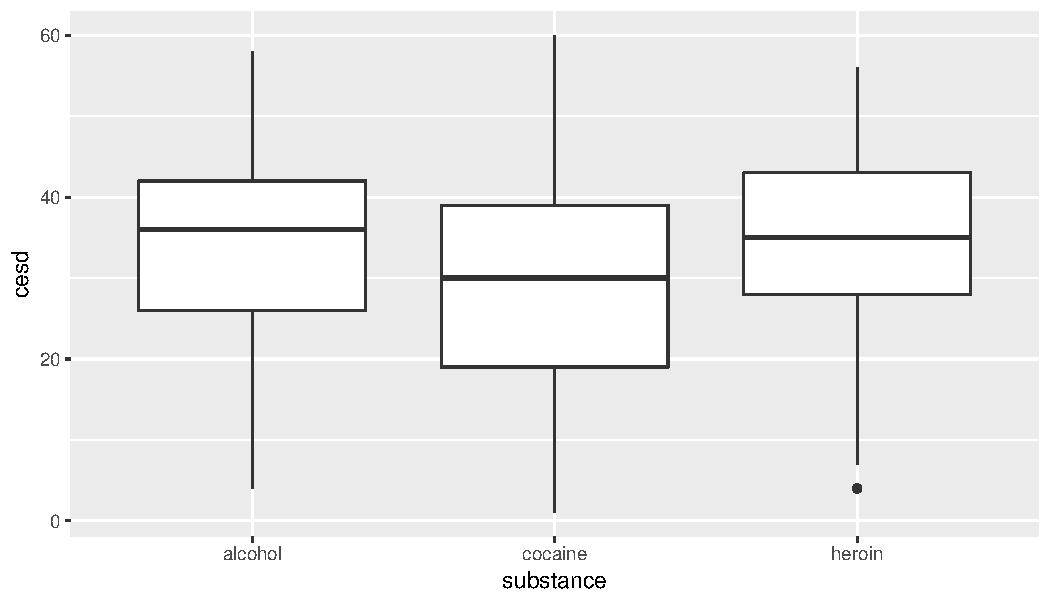
\includegraphics[width=\maxwidth]{figure/unnamed-chunk-1-1} 

\end{knitrout}

  \vspace{-0.5in}
  \item Using $\alpha = 0.05$, what is your decision regarding the viability of the null hypothesis?
  \item Write \emph{one} sentence summarizing what you've learned about the millenials and their opinions on same-sex marriage.  
  \vspace{0.5in}
\end{enumerate}


\paragraph{Exam 1 recap}

Since no one got 100\% I rescaled the exam to be out of 82 points. With that taken into account, most students scored between 79\% and 91\%. If your score is not what you would like, please make use of additional resources (e.g. Stats TAs, Spinelli Center tutoring, my office hours, study groups with fellow students, etc.)

\begin{itemize}
  \itemsep0em
  \item ``A" range: 74 points or above
  \item ``B" range: 66 - 73
  \item ``C" range: 58 - 65
  \item ``D" range: 50 - 67
\end{itemize}

I am implementing a bootstrap incentive for this exam. If you scored below a 66, you still have an opportunity to improve your grade. The \emph{threshold} for this exam is 66. If you score above the threshold for \emph{either of the next two exams}, your score on \emph{this} exam will be raised to 66/82, or 80\%.

% \newpage
% 
% \subsection*{Instructor's Notes}
% 
% 
% <<>>=
% pdata(~ prop, q = 0.66, data = p_hats, lower.tail = FALSE) * 2
% @
% 
% 
% 
% <<>>=
% dbinom(0,c(1:5),.5)
% @


\end{document}
